\subsection{SVD Field Translations}

In order to uniquely label M2L interactions we introduce transfer vectors $t = (t_1, t_2, t_3)$, $t \in \mathbb{Z}^3$. They describe the relative positioning of two boxes, $X$ and $Y$, in a hierarchical tree and are computed from their centres $t = \frac{c_x - c_y}{w}$ where $w$ is the box width.

Consider the application of $T^{M2L}$, to a given multipole expansion $q$, where our goal is to compute the check potential $\phi$,

\begin{flalign}
    \phi = T^{M2L} q
\end{flalign}


As $T^{M2L}$ is known to be low-rank, it can be optimally approximated with an SVD,

\begin{flalign}
    \tilde{\phi} = U_k \Sigma_k V_k^T q
\end{flalign}

where $k$ indicates the rank of $T^{M2L}$, i.e. the smallest non-zero singular value. This can be shown to be an optimal approximation to $K$ \cite{Trefethen1997}. For homogenous, translationally invariant kernels we see from Table \ref{table:chpt:2:sec:1:m2l_optimisations} that there are at most 316 unique translation vectors corresponding to $T^{M2L}$ operations in $\mathbb{R}^3$. Stacking their corresponding discrete matrices column wise,

\begin{flalign}
    T^{M2L}_{\text{fat}} &= \left [ T^{M2L}_1, ..., T^{M2L}_{316} \right ] \\
    &= U \Sigma \left [ V^{T}_1, ..., V^{T}_{316} \right ]
    \label{eq:chpt:3:sec:1:subsec:1:m2l_fat}
\end{flalign}

or row-wise,

\begin{flalign}
    T^{M2L}_{\text{thin}} &= \left [ T^{M2L}_1; ...; T^{M2L}_{316} \right ] \\
    &= \left [ R^{T}_1; ...; R^{T}_{316} \right ]  \Lambda S^T
    \label{eq:chpt:3:sec:1:subsec:1:m2l_thin}
\end{flalign}


we note that,

\begin{flalign}
    T^{M2L}_{\text{thin}}  = (T^{M2L}_{\text{fat}})^T
\end{flalign}

for such kernels which are symmetric. Having computed these two SVDs we can reduce the application cost of a given $T^{M2L}_i$ between two boxes,

\begin{flalign}
    T^{M2L}_i q = R_i\Lambda S^T q
    \label{eq:chpt:3:sec:1:subsec:1:single_svd}
\end{flalign}

Using the fact that $S$ is unitary, i.e. $S^TS = I$, we can insert this into equation (\ref{eq:chpt:3:sec:1:subsec:1:single_svd}) to find,

\begin{flalign}
    T^{M2l}_{i} q &= R^{(i)}\Lambda S S^T S^T q \\
    &= T^{M2L}_{i} SS^T q \\
    &= U \Sigma V^{T}_i SS^T q \\
\end{flalign}


Now using that $U$ is also unitary such that $U^TU = I$, we find

\begin{flalign}
    T^{M2L}_i q &= UU^T U \Sigma V^{T}_i SS^T q \\
    &= U [U^T U \Sigma V^{T}_i S] S^T q \\
    &= U[U^T T^{M2L}_i S] S^T q
\end{flalign}


The bracketed terms can be calculated using the rank $k$ approximation from the SVD,

\begin{flalign}
    [U^T T^{M2L}_i S] &= \Sigma V^{T}_i S\\
    &= U^T R_{i} \Lambda
    \label{eq:chpt:3:sec:1:subsec:1:compressed_m2l}
\end{flalign}


We call equation (\ref{eq:chpt:3:sec:1:subsec:1:compressed_m2l}) the \textit{compressed $T^{M2L}$ operator}.

\begin{flalign}
    C^k_i = U^T T^{M2L}_i S
    \label{eq:chpt:3:sec:1:subsec:1:compressed_m2l_2}
\end{flalign}

This matrix can be precomputed for each unique interaction. Therefore in the kernels considered in this exposition, it must be computed at most 316 times, with corresponding pre-computations for kernels with different properties.

The application of $T^{M2L}$ can now be broken down into four steps.


\begin{enumerate}
    \item Find the `compressed multipole expansion'
    \[
    q_c = S^T q
    \]
    \item Compute the `compressed check potential', where the sum is taken over all boxes which have an applicable $T^{M2L}$ operator, ie its interaction list.
    \[
    \phi_c = \sum C^k_i q_c
    \]
    \item Post process to recover an uncompressed check potential
    \[
    \phi = U \phi_c
    \]
    \item Finally, calculate the local expansion from the check potential as done previously in Section \ref{chpt:2:sec:2}.
\end{enumerate}


The rank behaviour of $T^{M2L}$ has been assumed to be low-rank throughout this thesis, and therefore amenable to compression. However it remains an open question as to the exact rank behaviour of a given kernel in practice. This has consequences for real implementations, as if we are able to effectively cut-off the rank $k$ with $\kappa \ll k$ we may be able to reduce the complexity of the SVD based scheme $T^{M2L}$ further. Figure \ref{fig:chpt:3:sec:1:subsec:1:rank_experiment} shows the effective rank behaviour of the Laplace kernel for different expansion orders. In this experiment we calculated the number of singular values greater than a threshold of $10^{-10}$ for all 316 unique transfer vectors for the Laplace kernel. We see that that width of the distribution has a strong relationship with the expansion order $P$, however the median rank remains approximately the same regardless of the expansion order. This implies that their is some dependency of the low-rank approximation for smaller transfer vectors for larger expansion orders. Analytical investigations could reveal what this is explicitly, as this would inform the cut-off value taken for $\kappa$, as it is an open question to what this behaviour is explicitly. Understanding this would inform practical implementations of an SVD based approach to sparsifying $T^{M2L}$.

\begin{figure}
    \centering
    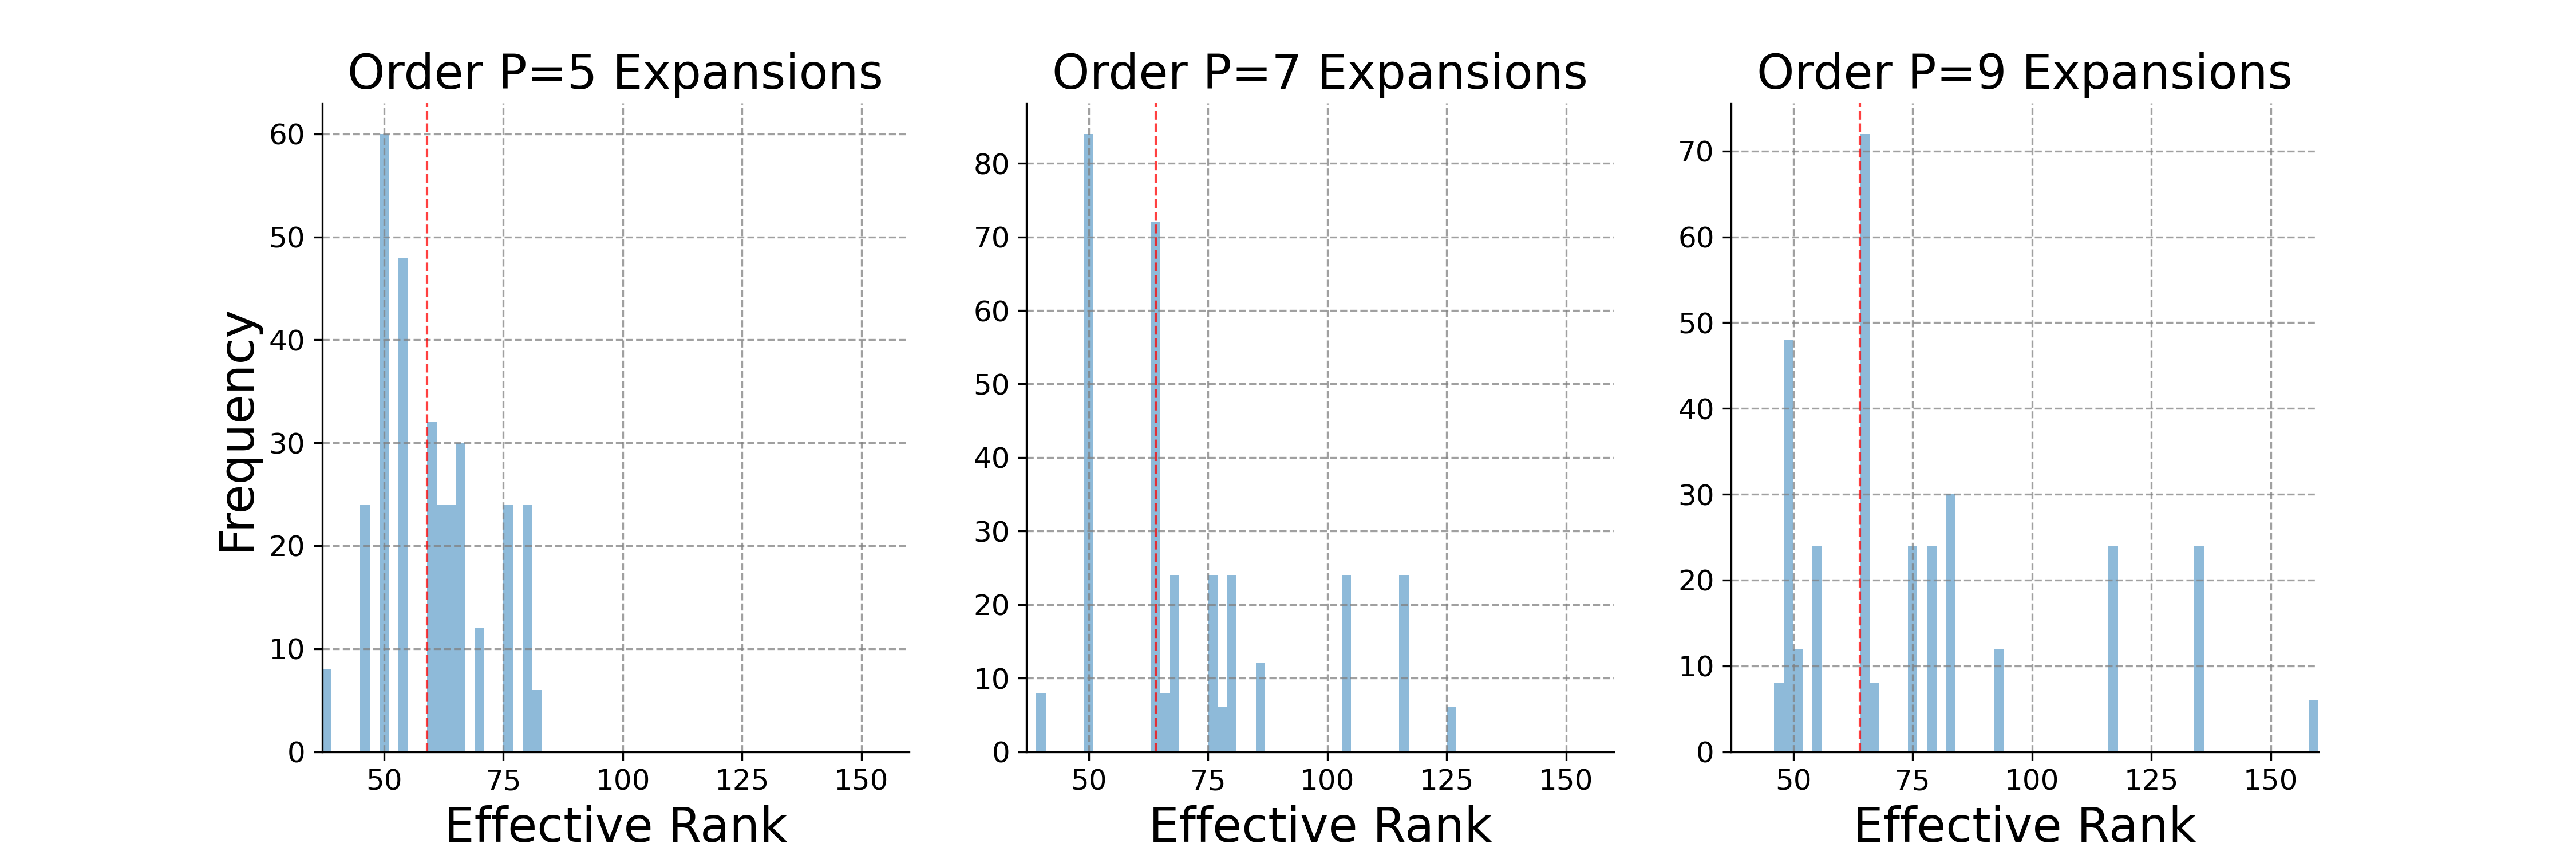
\includegraphics[width=\textwidth]{images/ch_3/rank_histogram.png}
    \caption{Rank behaviour of $T^{M2L}$ computed for the Laplace kernel at different expansion orders presented as a distribution over the 316 unique transfer vectors for this kernel. We estimated the ranks of each matrix by counting the number of singular values greater than $10^{-10}$. The red dashed line indicates a median rank, for $P=5$ it was found to be 59. for $P=7$ and 9 it was found to be 64.}
    \label{fig:chpt:3:sec:1:subsec:1:rank_experiment}
\end{figure}

Practical implementations can re-formulate the SVD based scheme to increase the computational intensity\footnote{The computational intensity is short hand for the ratio of computations to memory accesses, i.e. flops/bytes.} of the operation. As presented above, each box $B$ will have to compute $T^{M2L}$ for each box in its relevant interaction list, up to 189 times in $\mathbb{R}^3$. For each of these applications, $B$ will have to look up the appropriate compressed $T^{M2L}$ from memory in this naive scheme. Matrix vector products are handled by BLAS level 2 operations, however by taking advantage of BLAS level 3 operations we can increase the ratio of computations to memory accesses. We do so in our implementation by blocking together \textit{all} the right hand sides, i.e. multipole expansions, which share a given translation vector $t$ and compute their compressed check potentials in a single matrix-matrix product. This has a dramatic effect on the runtime of our software as shown in Figure \ref{fig:chpt:3:sec:1:subsec:1:svd_m2l}.

\begin{figure}
    \centering
    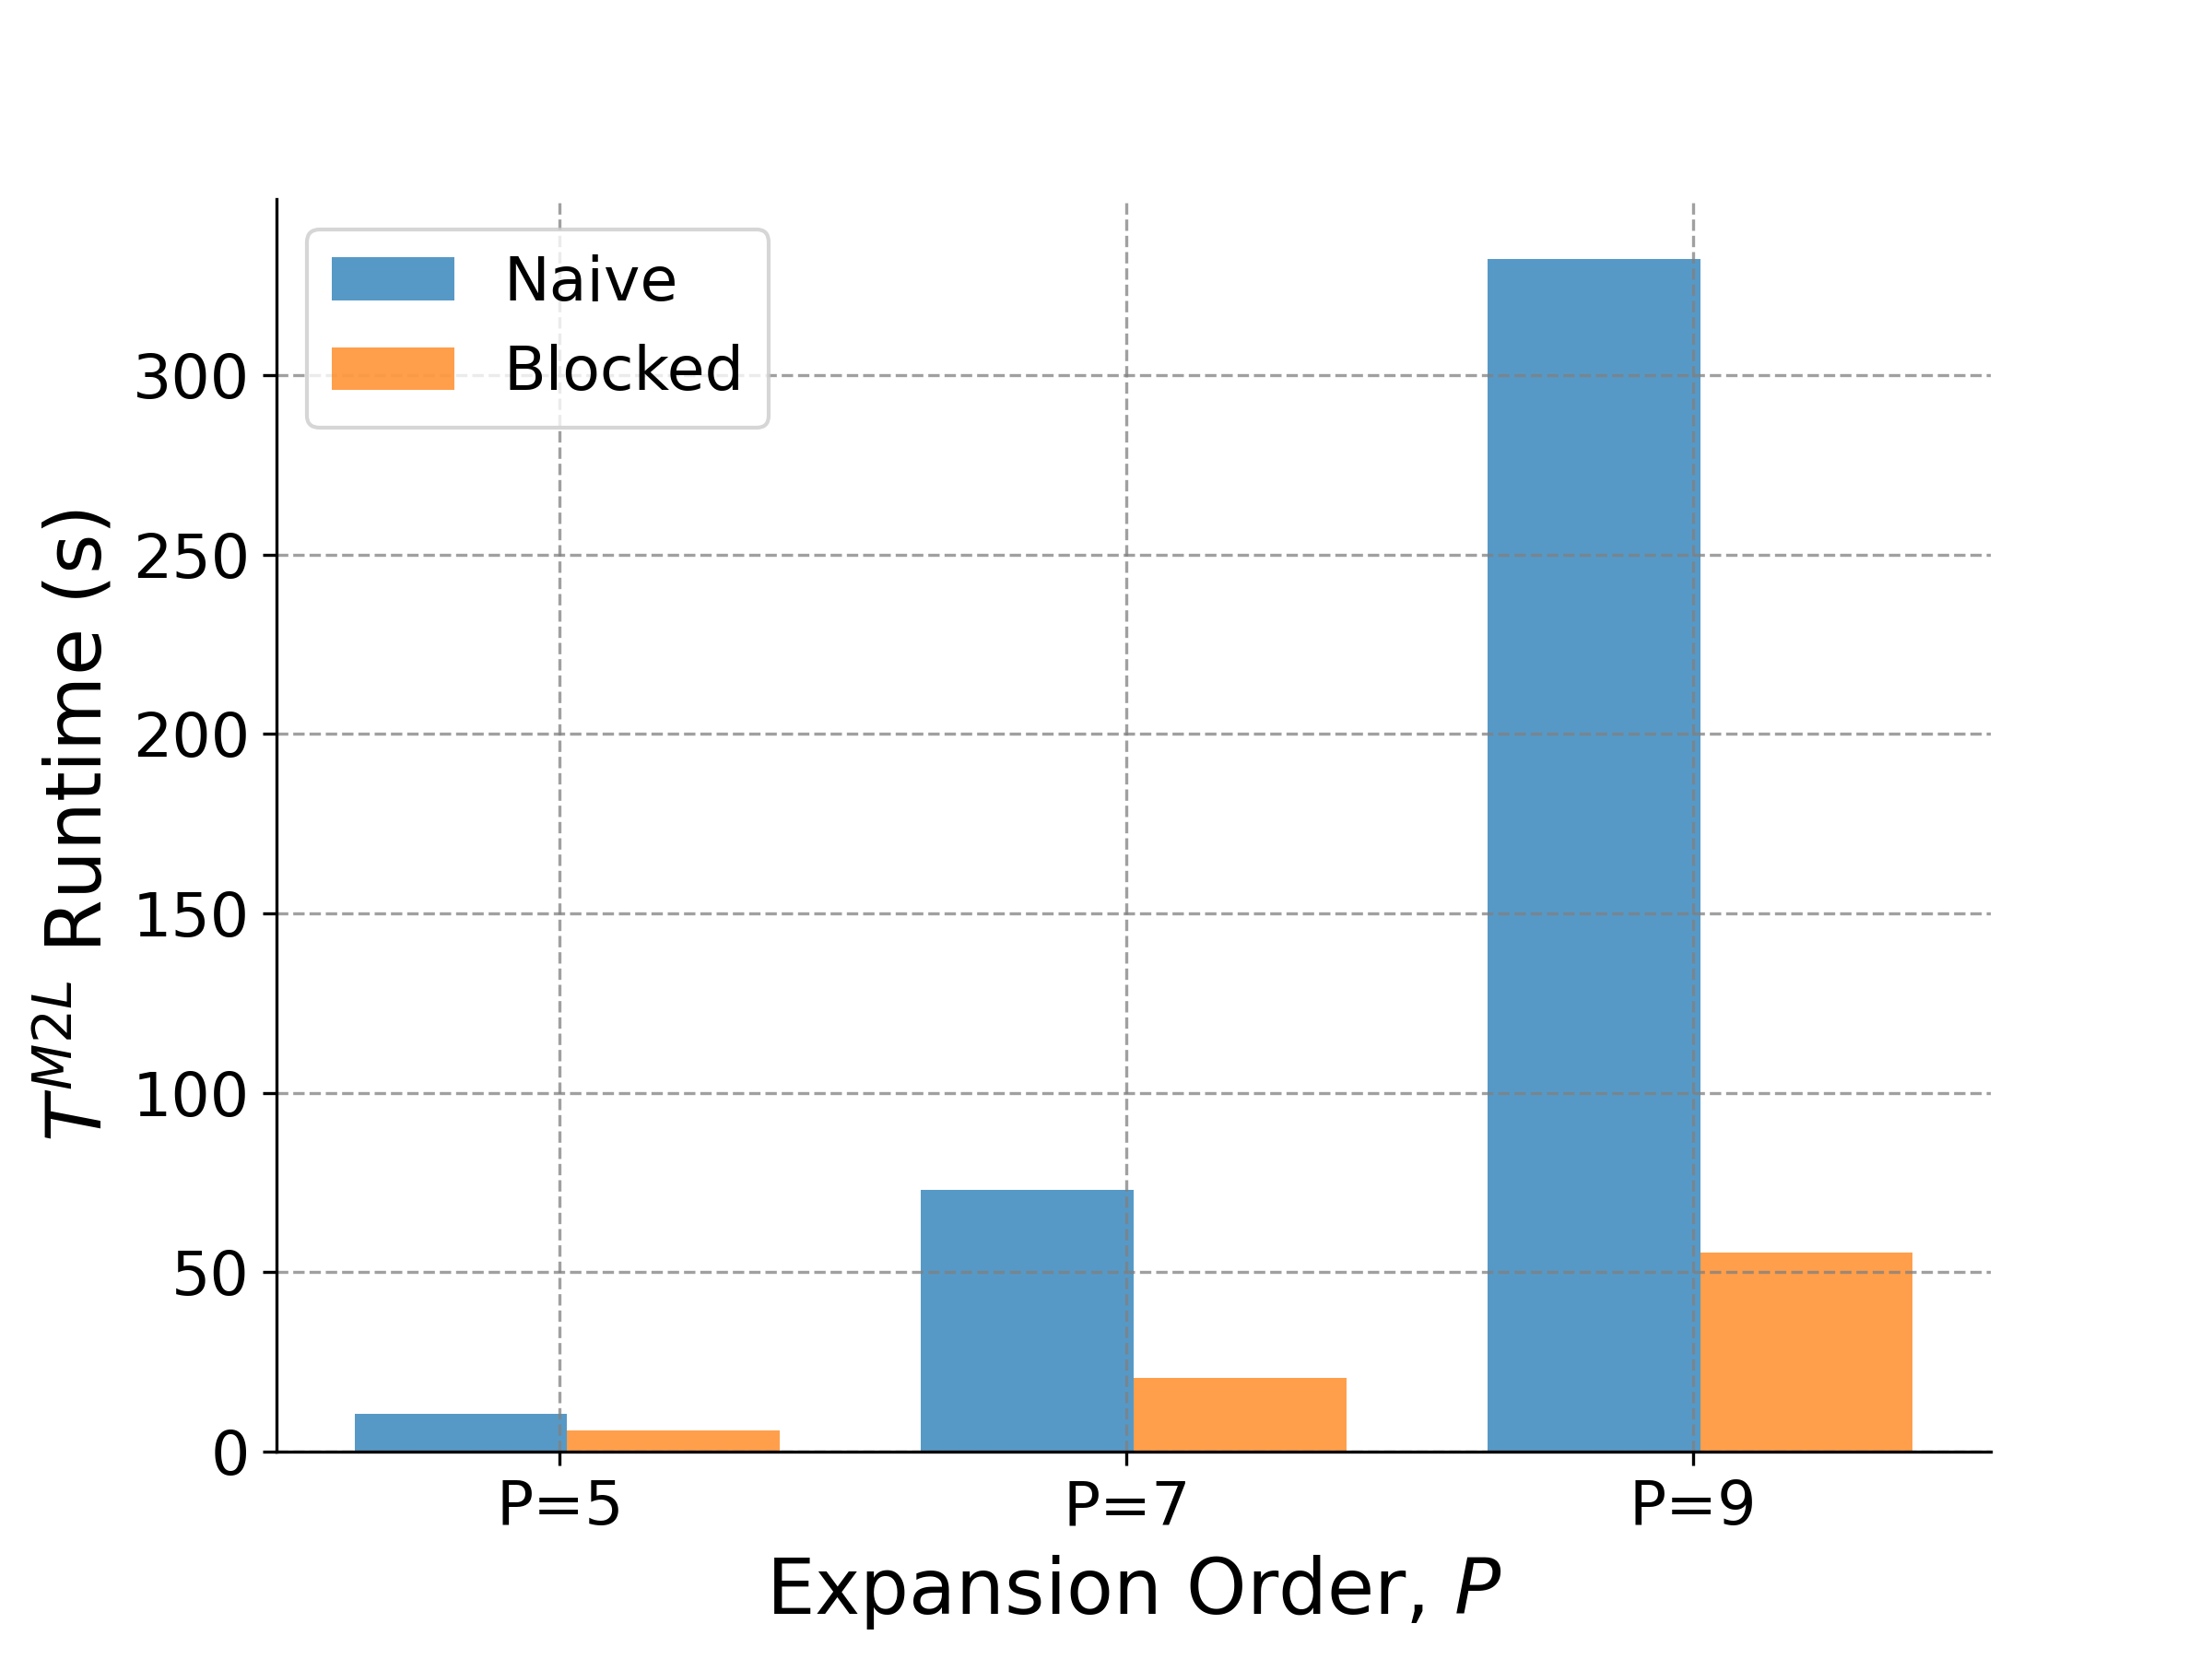
\includegraphics[width=0.6\textwidth]{images/ch_3/svd_m2l.png}
    \caption{Here we illustrate two schemes for computing $T^{M2L}$ in Rusty Field. The `Naive' scheme performs a parallel loop over the boxes at each level, looks up their associated $T^{M2L}$ and computes check potentials as a matrix-vector product. The blocking scheme uses the re-organisation outlined above to block together $T^{M2L}$s corresponding for all source/target boxes at a given level with matching transfer vectors, and thus computing a matrix-matrix product. Here we don't choose a cutoff rank $\kappa$, and all $T^{M2L}$ matrices are left uncompressed. Experiments are taken on a 6 core Intel i7-9750 processor using Open BLAS, we report maximum runtimes over 5 runs
    for each set of parameters.}
    \label{fig:chpt:3:sec:1:subsec:1:svd_m2l}
\end{figure}

We note that the precomputation for this approach relies on an SVD of two relatively large matrices in (\ref{eq:chpt:3:sec:1:subsec:1:m2l_fat}) and (\ref{eq:chpt:3:sec:1:subsec:1:m2l_thin}) where we use the `greedy' DGESVD provided by LAPACK. For the Laplace kernel, which is translationally invariant and homogenous, precomputation times are shown in Figure \ref{fig:chpt:3:sec:1:subsec:1:svd_m2l_precomputation}. However, for kernels which are translationally invariant but not homogenous, these must be computed for each level of the octree which can have a significant impact on setup time for the FMM, dominating the tree setup time as well as the algorithm runtime. This could be alleviated with alternative implementations that make use of randomised algorithms, which have been shown to have considerably faster runtimes for a given compression rank \cite{halko2011finding}, though we haven't explored this as of date.

\begin{figure}
    \centering
    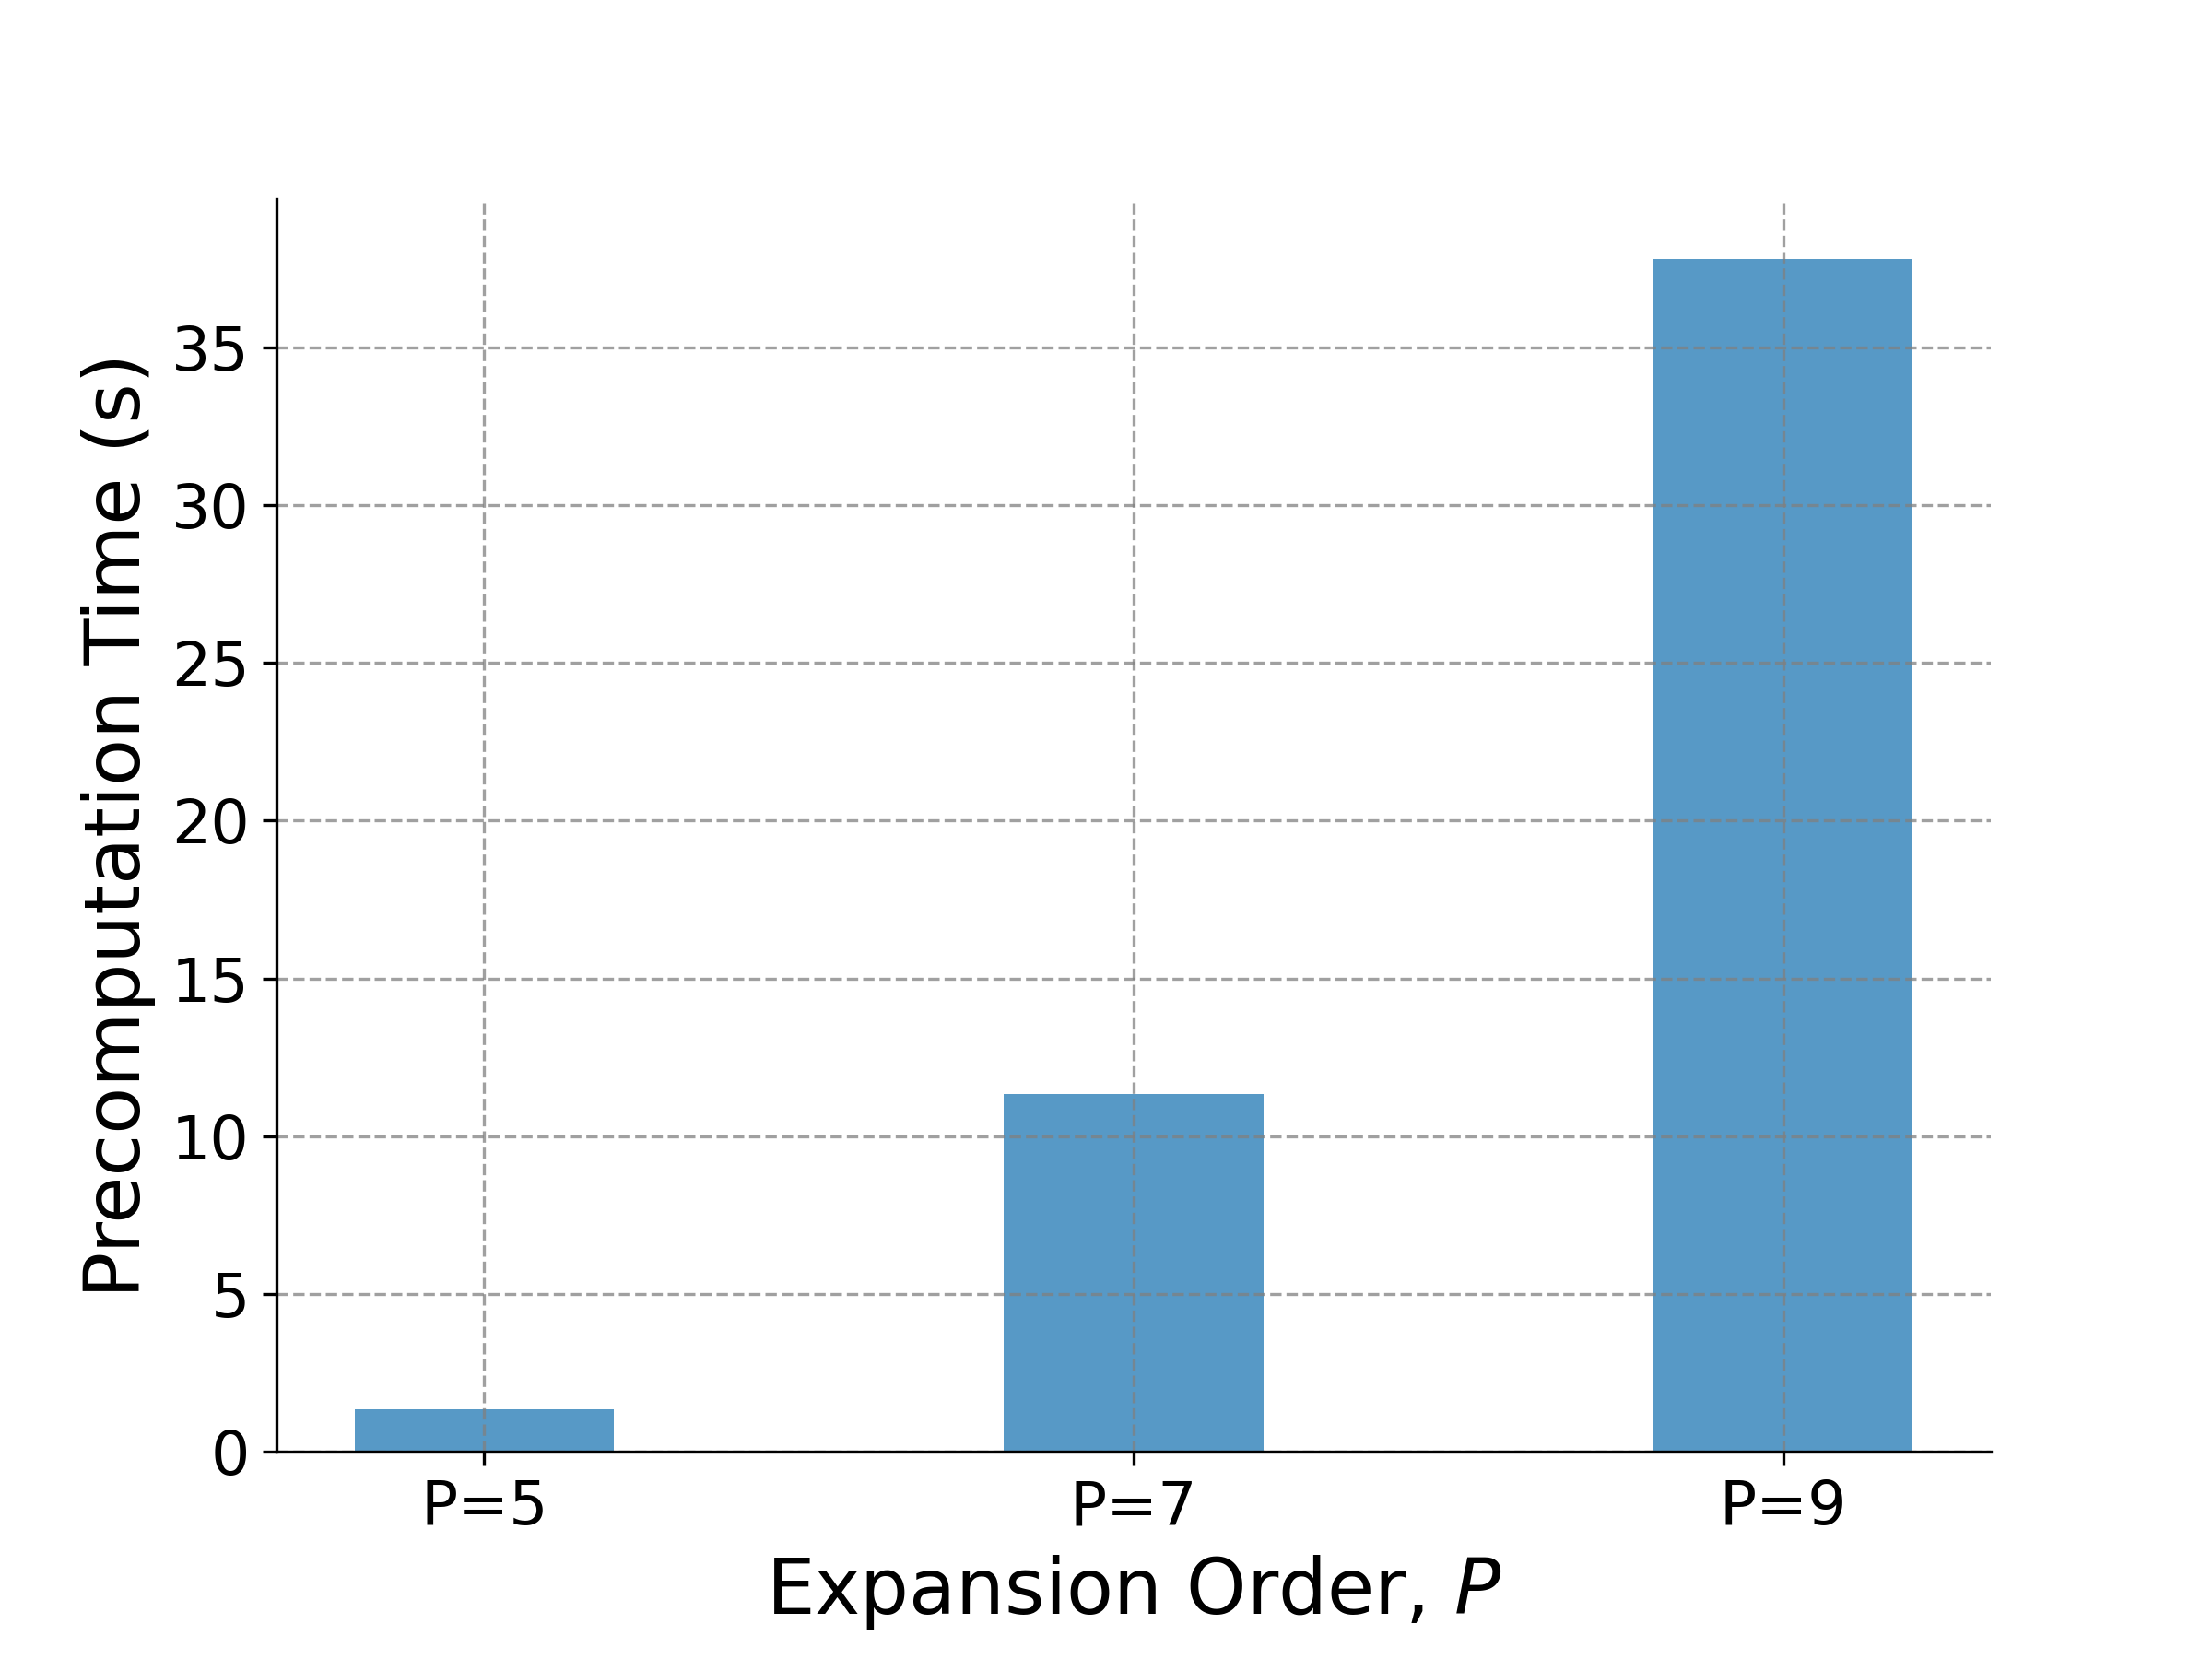
\includegraphics[width=0.6\textwidth]{images/ch_3/svd_m2l_precomputation.png}
    \caption{Here we illustrate the precomputation time to compute the SVDs of $T^{M2L}$ for a selection of expansion orders. We observe that precomputation time can grow dramatically with increased expansion order, for $P=9$ precomputation rivals the runtime of $T^{M2L}$ (see fig. \ref{fig:chpt:3:sec:1:subsec:1:svd_m2l}). Experiments are taken on a 6 core Intel i7-9750 processor using Open BLAS, we report maximum runtimes over 5 runs
    for each set of parameters.}
    \label{fig:chpt:3:sec:1:subsec:1:svd_m2l_precomputation}
\end{figure}